

\section{Evaluation}
\label{sec:eval}
%
Radix-hash join and merge-sort join are two of the most popularly used parallel implementations of the inner join
operation. Both these algorithms involve partitioning the input data so that they can be efficiently distributed
to the participating processes. For example, in the radix-hash approach a tuple is assigned to a process based
on the hash output of the column-value on which the join operation is keyed. With this approach, tuples on
both relations that share the same hash value are always assigned to the same process. For every tuple in the
left-hand side of the join relation is matched against all the tuples of the right-hand side of the join relation. Fast
lookup data-structures like hash tables, or radix-trees (TRIE) can be used to organize the tuples within every
process. The initial distribution of data using hashing reduces the overall computation overhead by a factor of
the number of processes (n).
More recently (Barthels et al. 2015, 2017), there has been a concerted effort to implement JOIN operations on
clusters using an MPI backend. The commonly used radix-hash join and merge-sort join have been re-designed
for this purpose. Both these algorithms involve a hash-based partitioning of data so that they are be efficiently
distributed to the participating processes and are designed such that inter-process communication is minimized.
In both of these implementations one-sided communication is used for transferring data between process. With
one-sided communication the initiator of a data transfer request can directly access parts of the remote memory
and has full control where the data will be placed. Read and write operations are executed without any
involvement of the target machine. This approach of data transfer involves minimal synchronization between
particiapting processes and have been shown to scale better that traditional two-sided communication. The
implementation of parallel join has shown promising performance numbers; for example, the parallel join algorithm
of (Barthels et al. 2017) ran successfully at 4,096 processor cores with up to 4.8 terabytes of input data


\subsection{Datasets}
\label{sec:datasets}
Lorem ipsum dolar sit amat


\begin{figure*}[t]
	{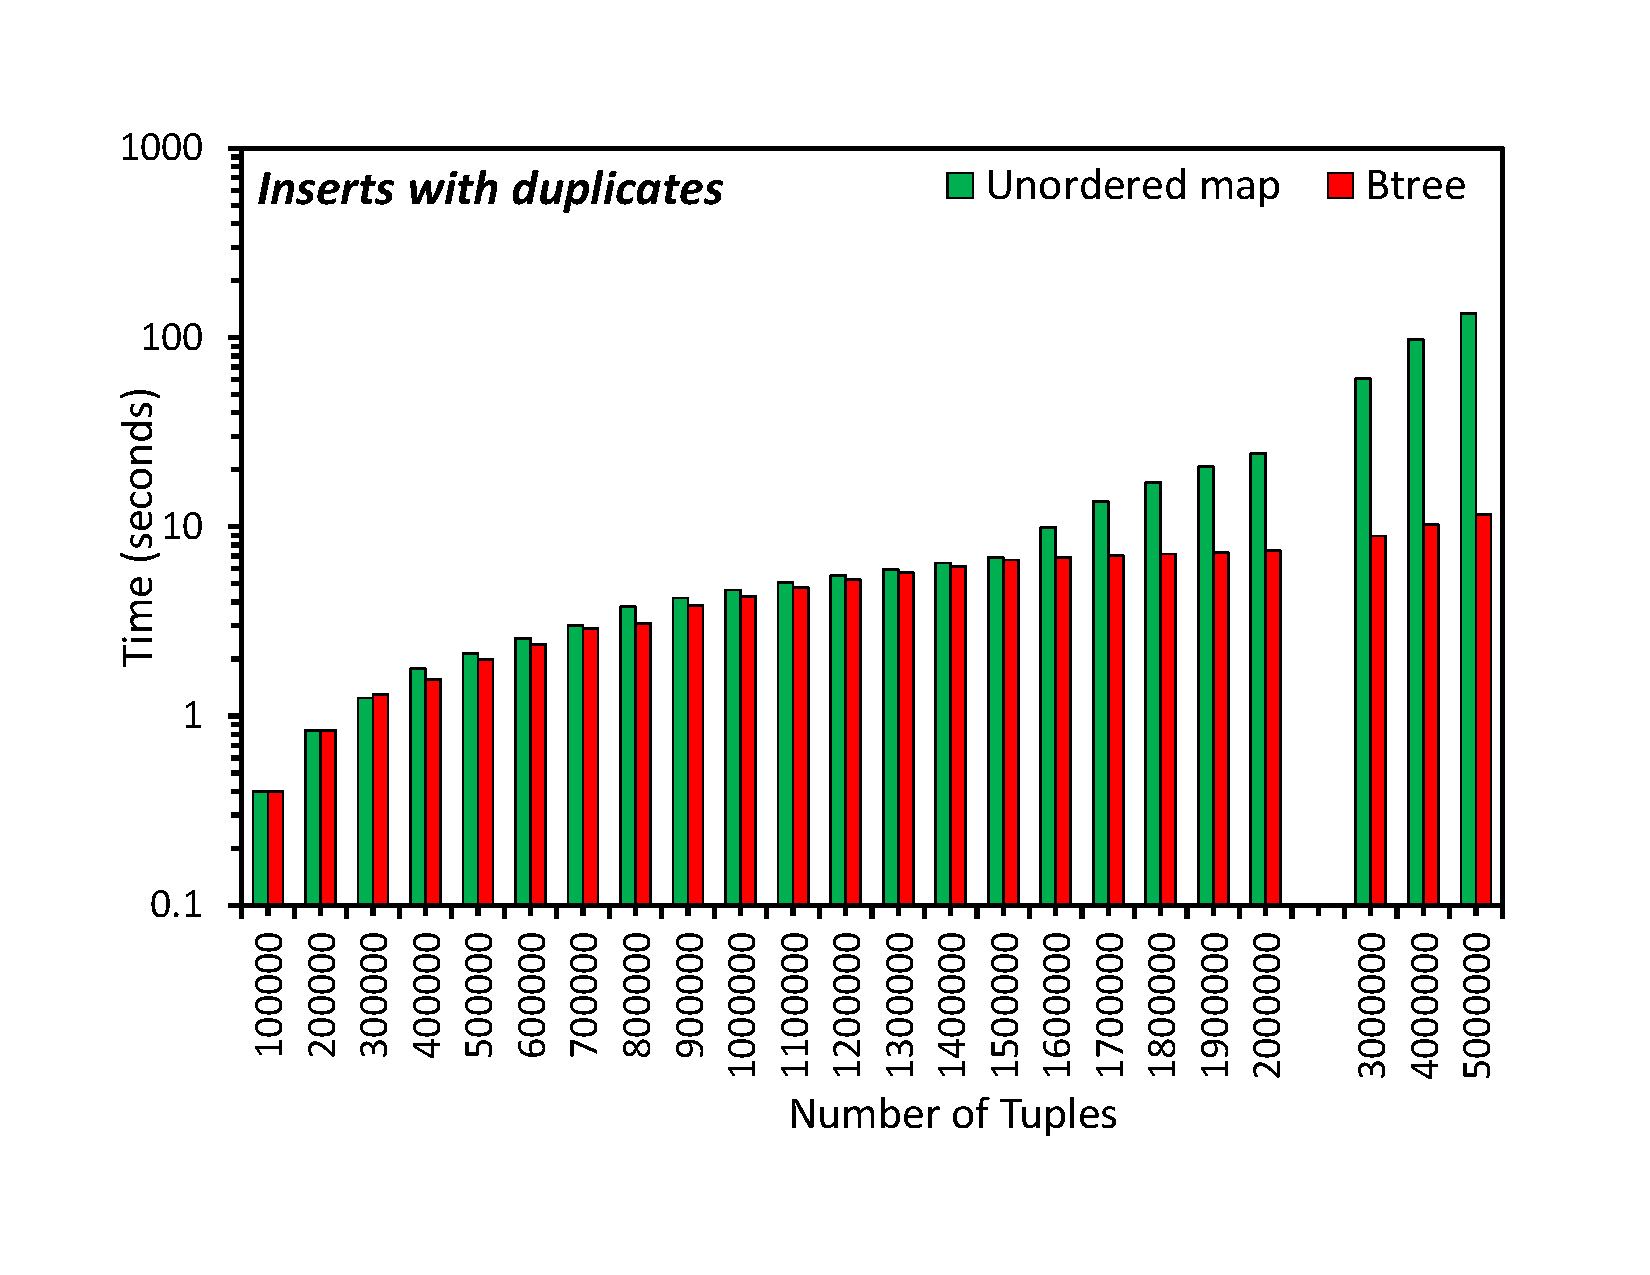
\includegraphics[width=.50\textwidth,  trim={0cm 0cm 0cm 0cm, 
			clip}]{results/inserts_with_duplicates.pdf}}\hfill%
	{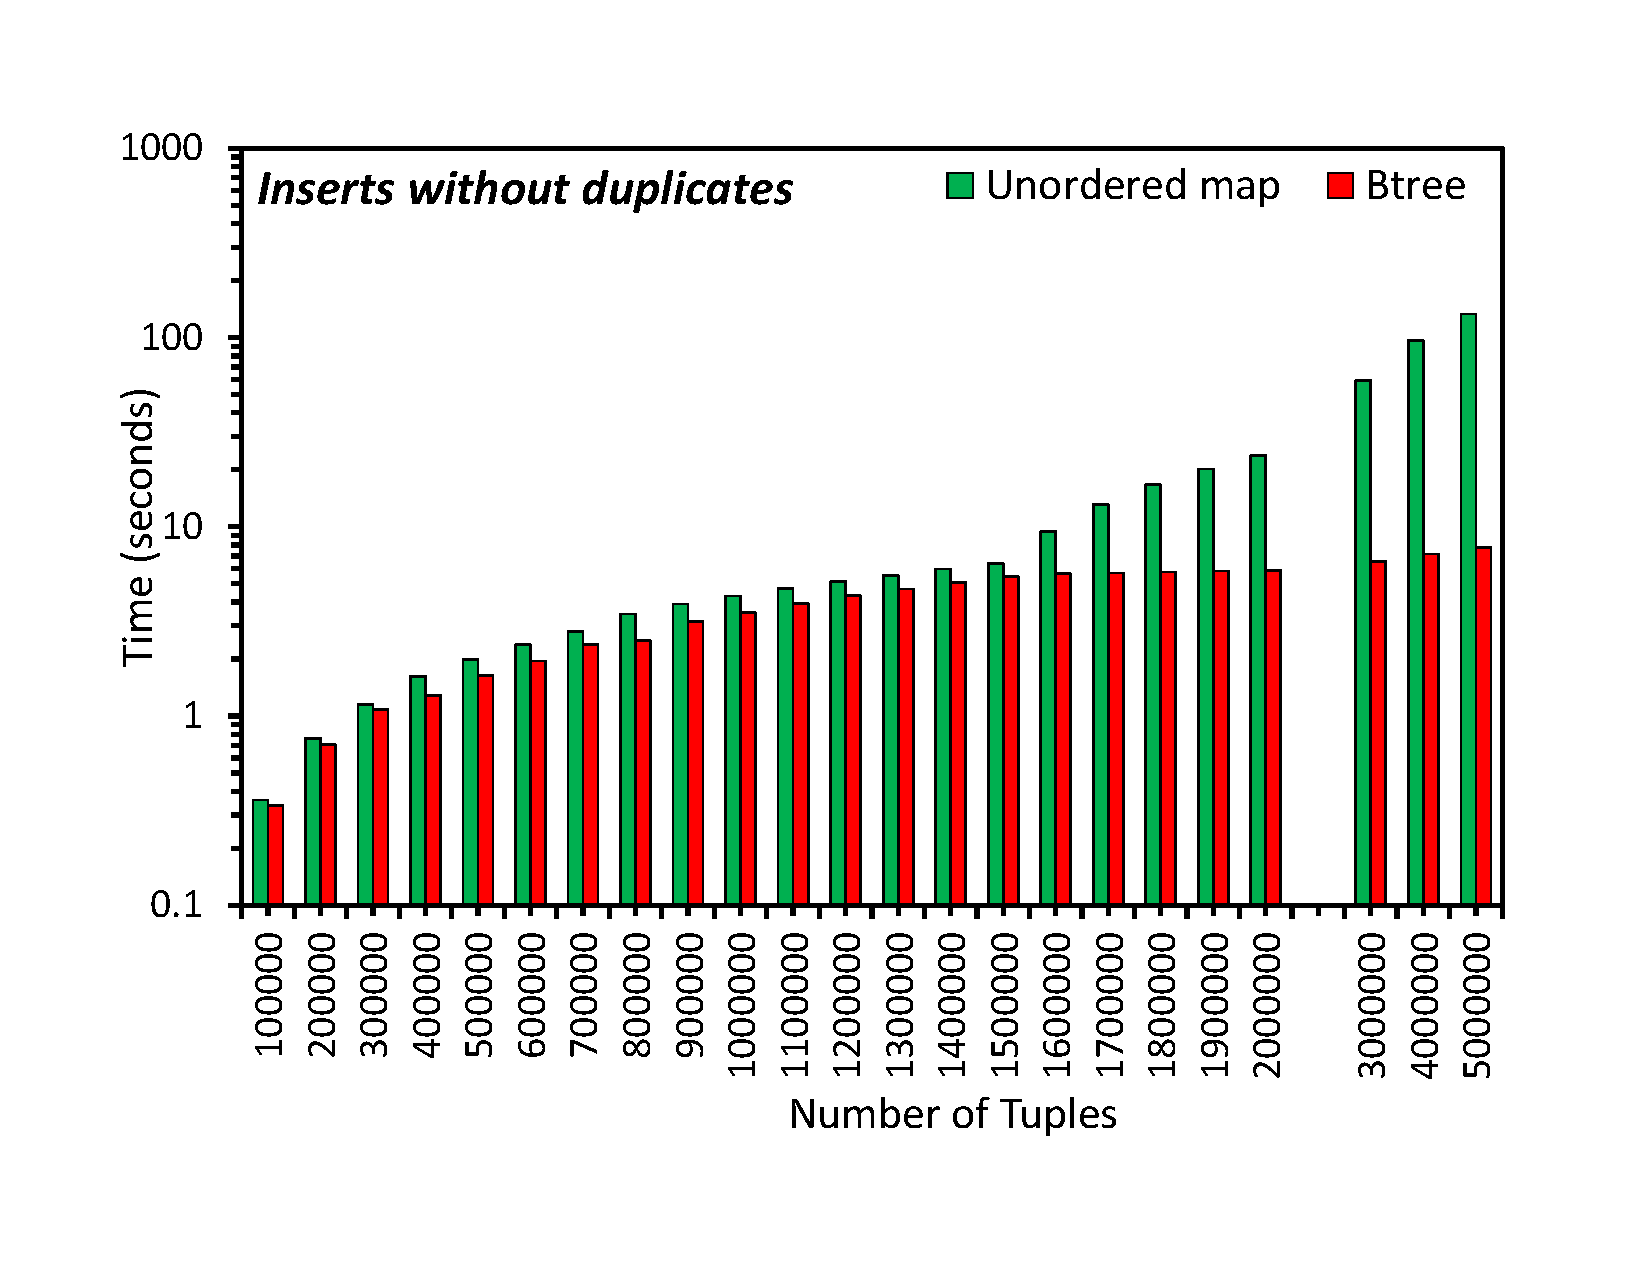
\includegraphics[width=.50\textwidth,  trim={0cm 0cm 0cm 0cm,
			clip}]{results/inserts_with_no_duplicates.pdf}}\hfill%
	\centering
	\caption{Performance evaluation of relation class implemented with btree and unordered map. (left) All tuples are distinct, (right) There are four copies of every tuple being inserted. Relation implemented with btree out-performs the unordered-map implementation.}
	\label{fig:tuple_inserts}
\end{figure*}


\begin{figure*}[t]
	{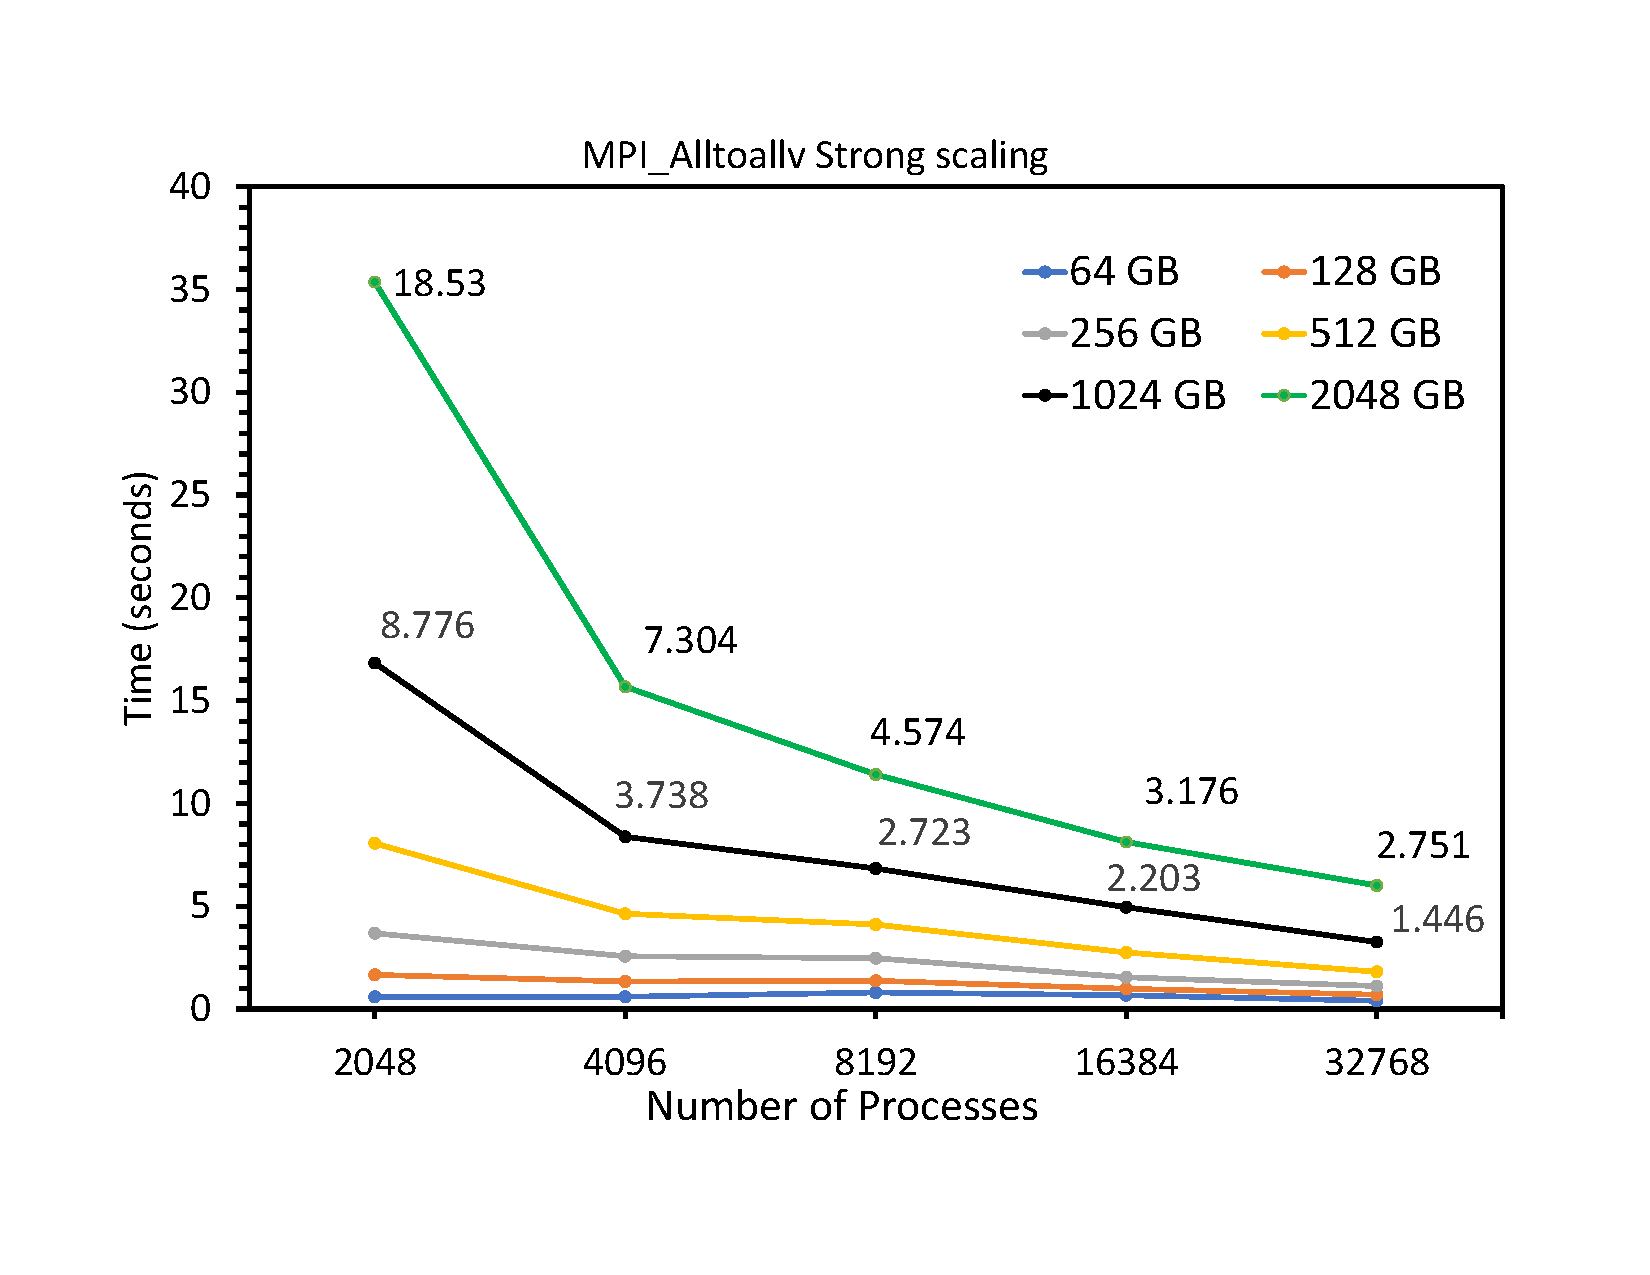
\includegraphics[width=.50\textwidth,  trim={0cm 0cm 0cm 0cm, 
			clip}]{results/all_to_all_strong.pdf}}\hfill%
	{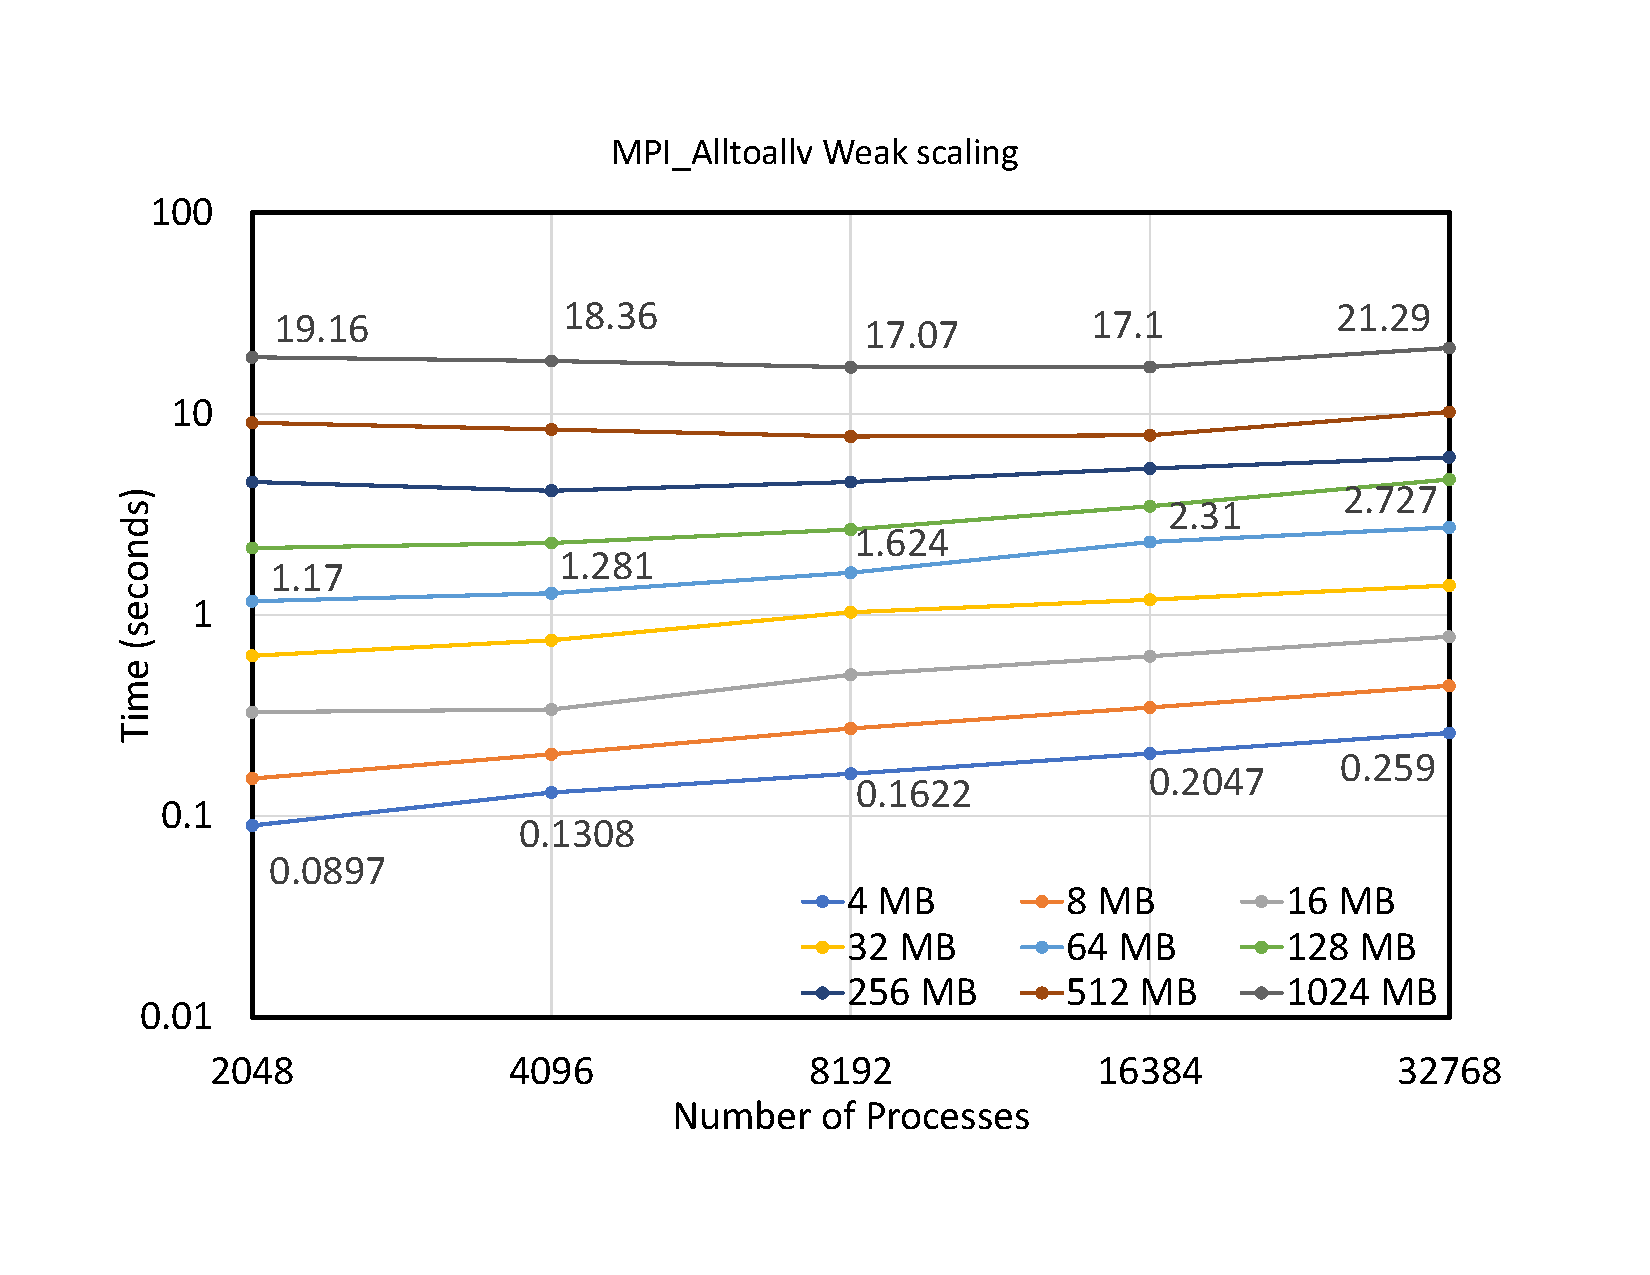
\includegraphics[width=.50\textwidth,  trim={0cm 0cm 0cm 0cm,
			clip}]{results/all_to_all_weak.pdf}}\hfill%
	\centering
	\caption{Strong (left) and Weak (right) scaling evaluation of MPI\_alltoallv function of MPI.}
	\label{fig:all_to_all}
\end{figure*}


\subsection{Relation}
\label{sec:relation}
Lorem ipsum dolar sit amat


\subsection{Parallel Union}
\label{sec:union}
Lorem ipsum dolar sit amat


\subsection{Parallel Join}
\label{sec:join}
Lorem ipsum dolar sit amat


\subsection{All to all communication}
\label{sec:ata}
Lorem ipsum dolar sit amat


\subsection{Transitive closure}
\label{sec:tc}

Computing the transitive closure of a graph involves repeated join operations until a fixed point is reached. We
use the previously discussed radix-hash join algorithm to distribute the tuples across all processes. The algorithm
can then be roughly divided into four phases: 1) Join 2) network communication 3) insertion 4) checking for a
fixed point. In our join phase every process concurrently computes the join output of the local tuples. In the next
phase every process sends the join output results to the relevant processes. This is a all-to-all communication
phase, which we implemet using MPI’s all to all routines. The next step involves inserting the join output result
received from the network to the output graph’s local partition. In the final step we check if the size of the
output graph changed on any process, if it does then we have not yet reached a fixed point and we continue to
another iteration of these 4 steps.
We performed a set of strong-scaling experiments to compute the transitive closure of graph with 412148
edges—the largest graph in the U. Florida Sparse Matrix set (Davis and Hu 2011). We used the Quartz supercomputer
at the Lawrence Livermore National Laboratory (LLNL). For our runs, we varied the number of processes
from 64 to 2048. A fixed point was attained after 2933 iterations, with the resulting graph containing 1676697415
edges. As can be seen in Figure 1, our approach takes 462 seconds at 64 cores and 235 seconds at 2048 cores, corresponds
to an overall efficiency of 6.25%. We investigated these timings further by plotting the timing breakdown
of by the four major components (join, network communication, join, fixed-point check) of the algorithm. We
observe (see Figure 2) that for all our runs the total time is dominated by computation rather than communication;
insert and join together tended to take up close to 90% of the total time. This is quite an encouraging result
as it shows that we are not bound primarily by the network bandwidth (at these scales and likely moderately
higher ones) and it gives us the opportunity to optimize the computation phase

\begin{figure*}[t]
	{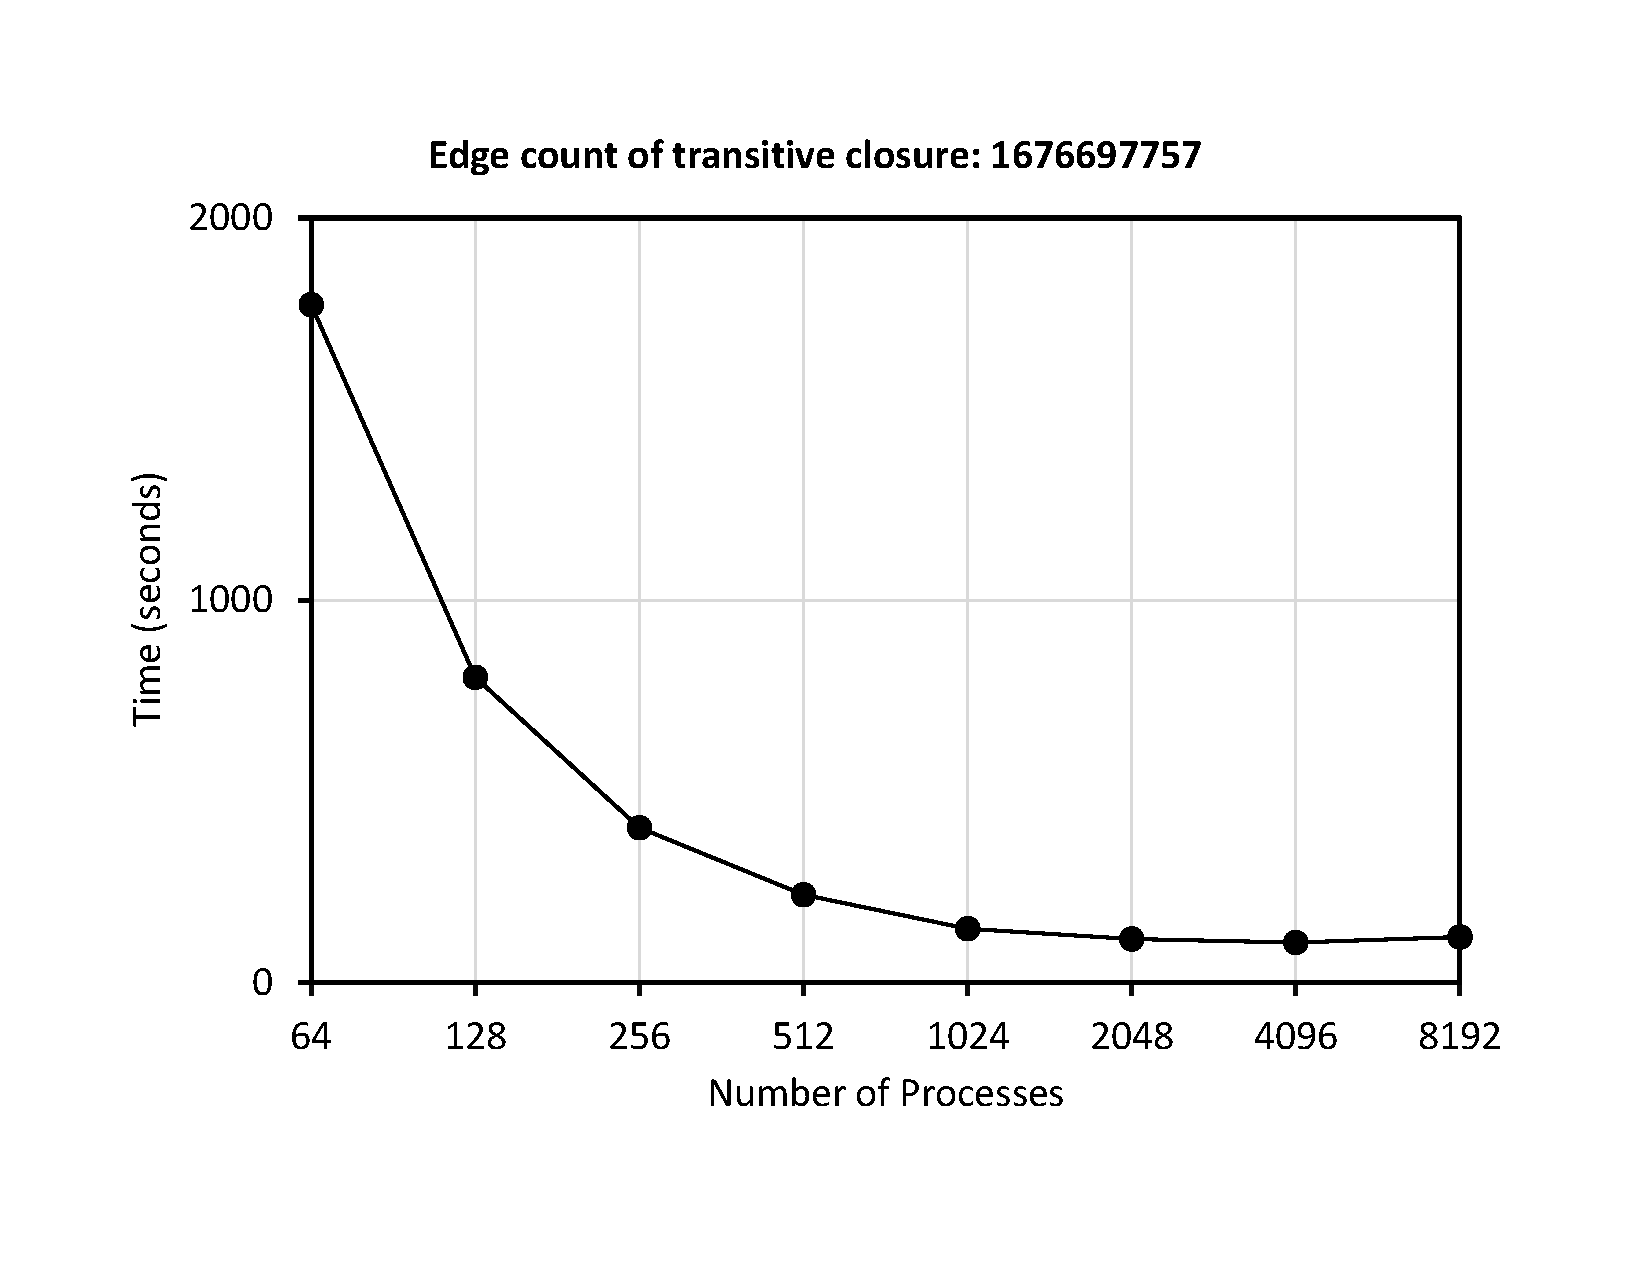
\includegraphics[width=.50\textwidth,  trim={0cm 0cm 0cm 0cm, 
			clip}]{results/TC_1_6Billion.pdf}}\hfill%
	{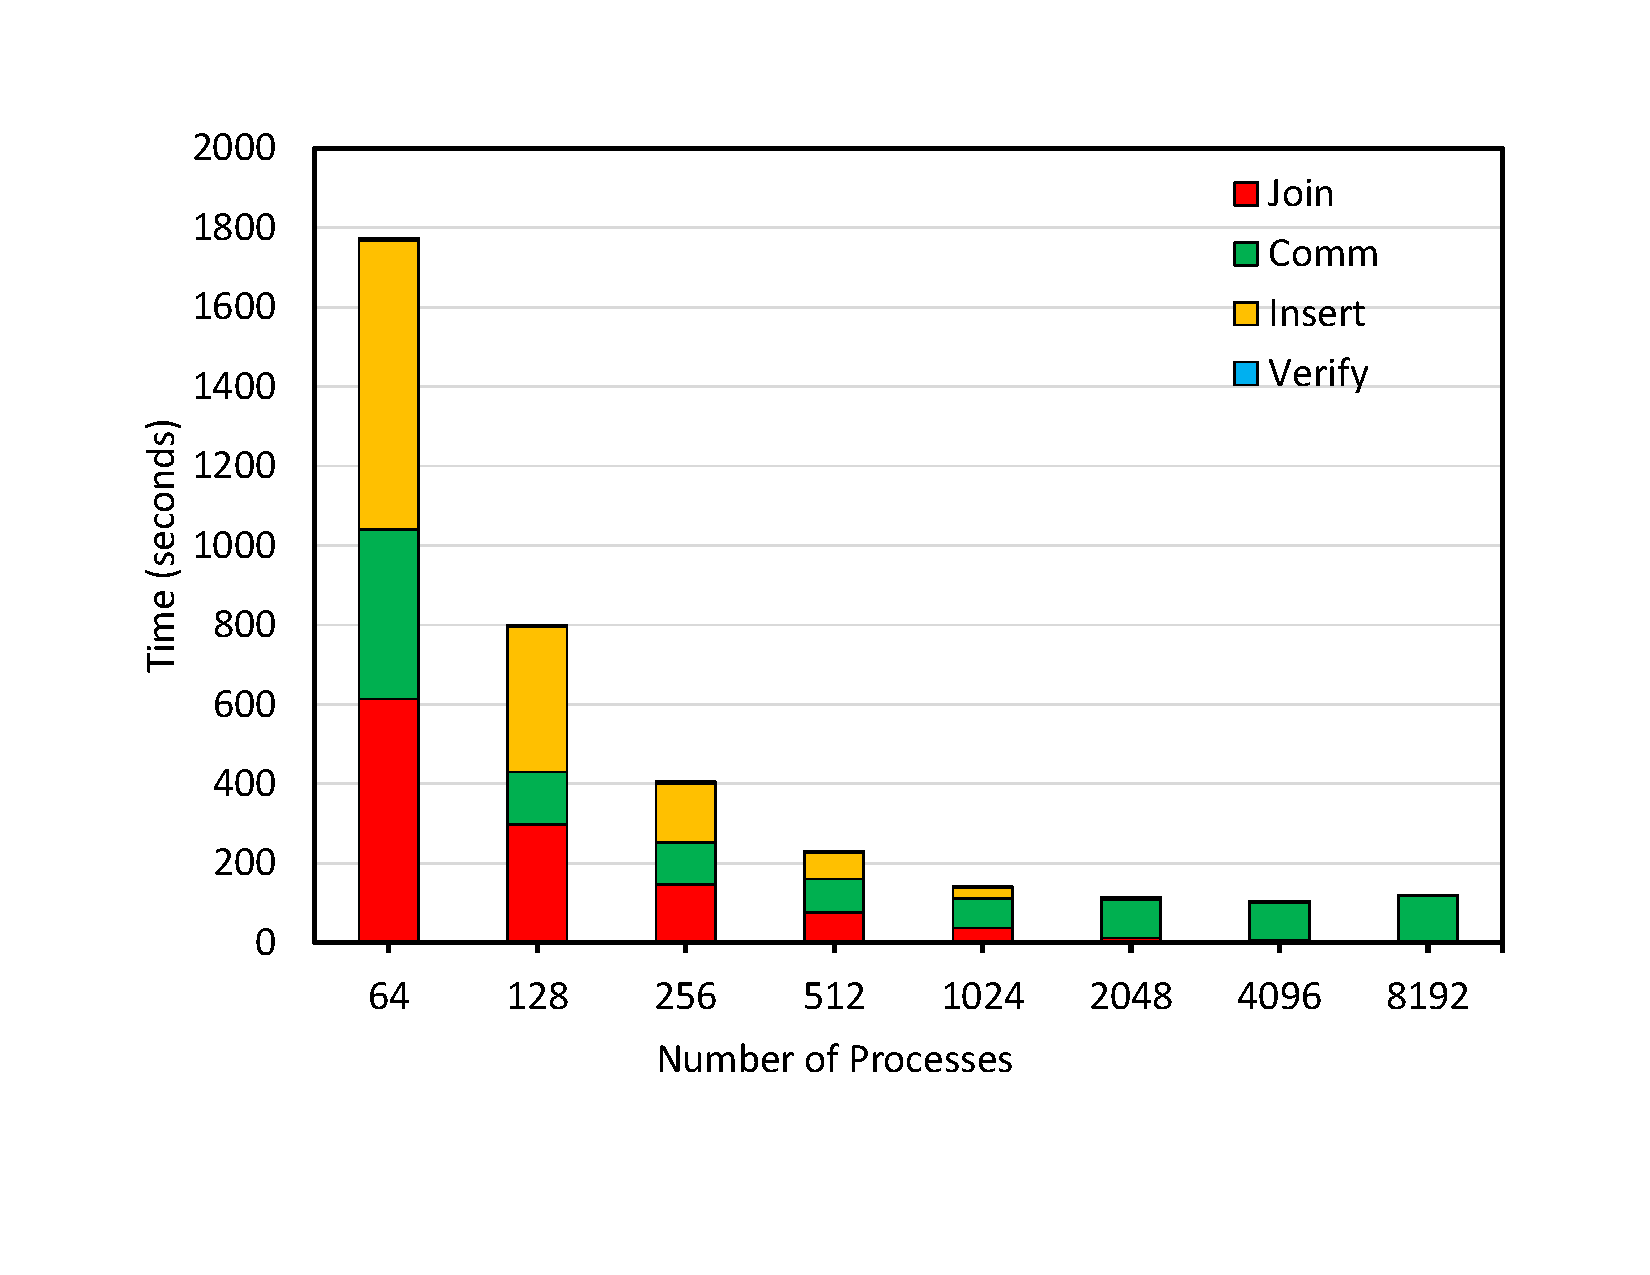
\includegraphics[width=.50\textwidth,  trim={0cm 0cm 0cm 0cm,
			clip}]{results/TC_1_6Billion_breakdown.pdf}}\hfill%
	\centering
	\caption{Transitive closure of a graph with X edges.}
	\label{fig:tc_small}
\end{figure*}


\begin{figure*}[t]
	{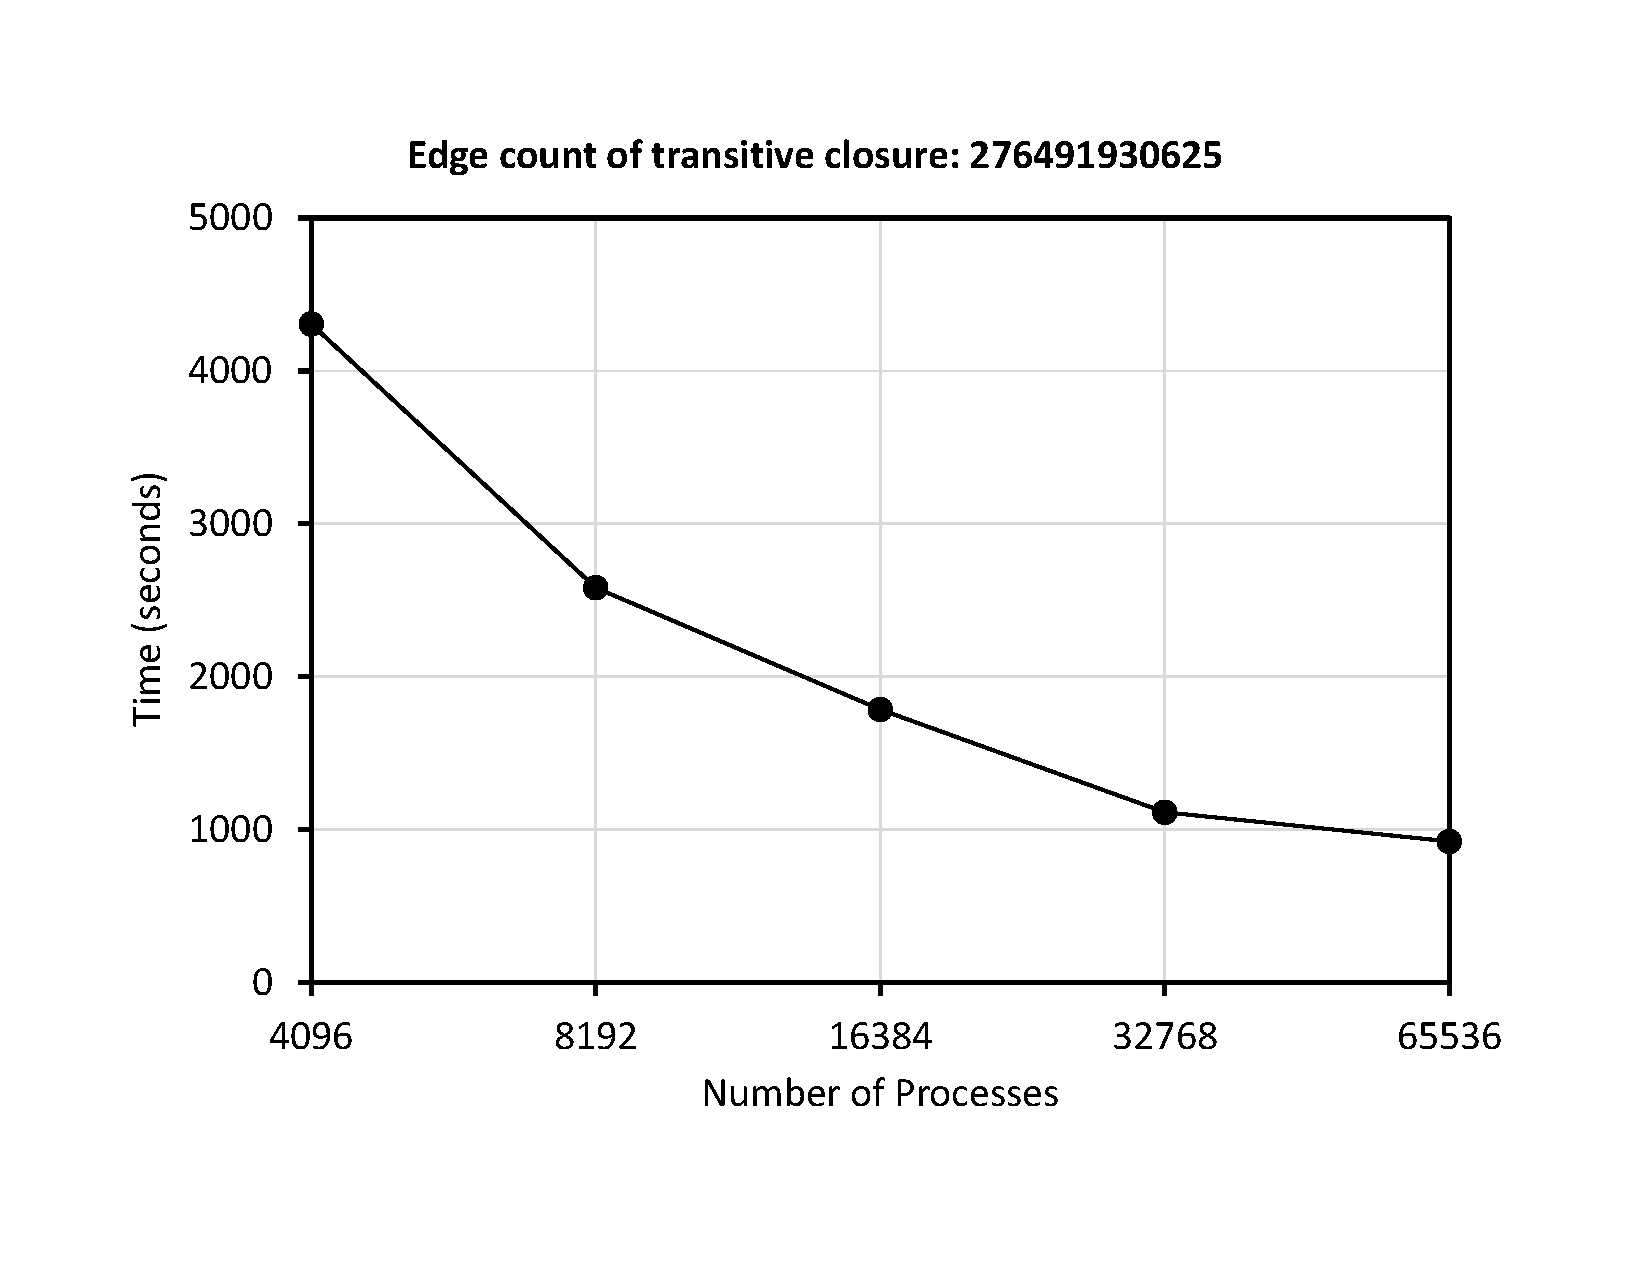
\includegraphics[width=.50\textwidth,  trim={0cm 0cm 0cm 0cm, 
			clip}]{results/TC_260Billion.pdf}}\hfill%
	{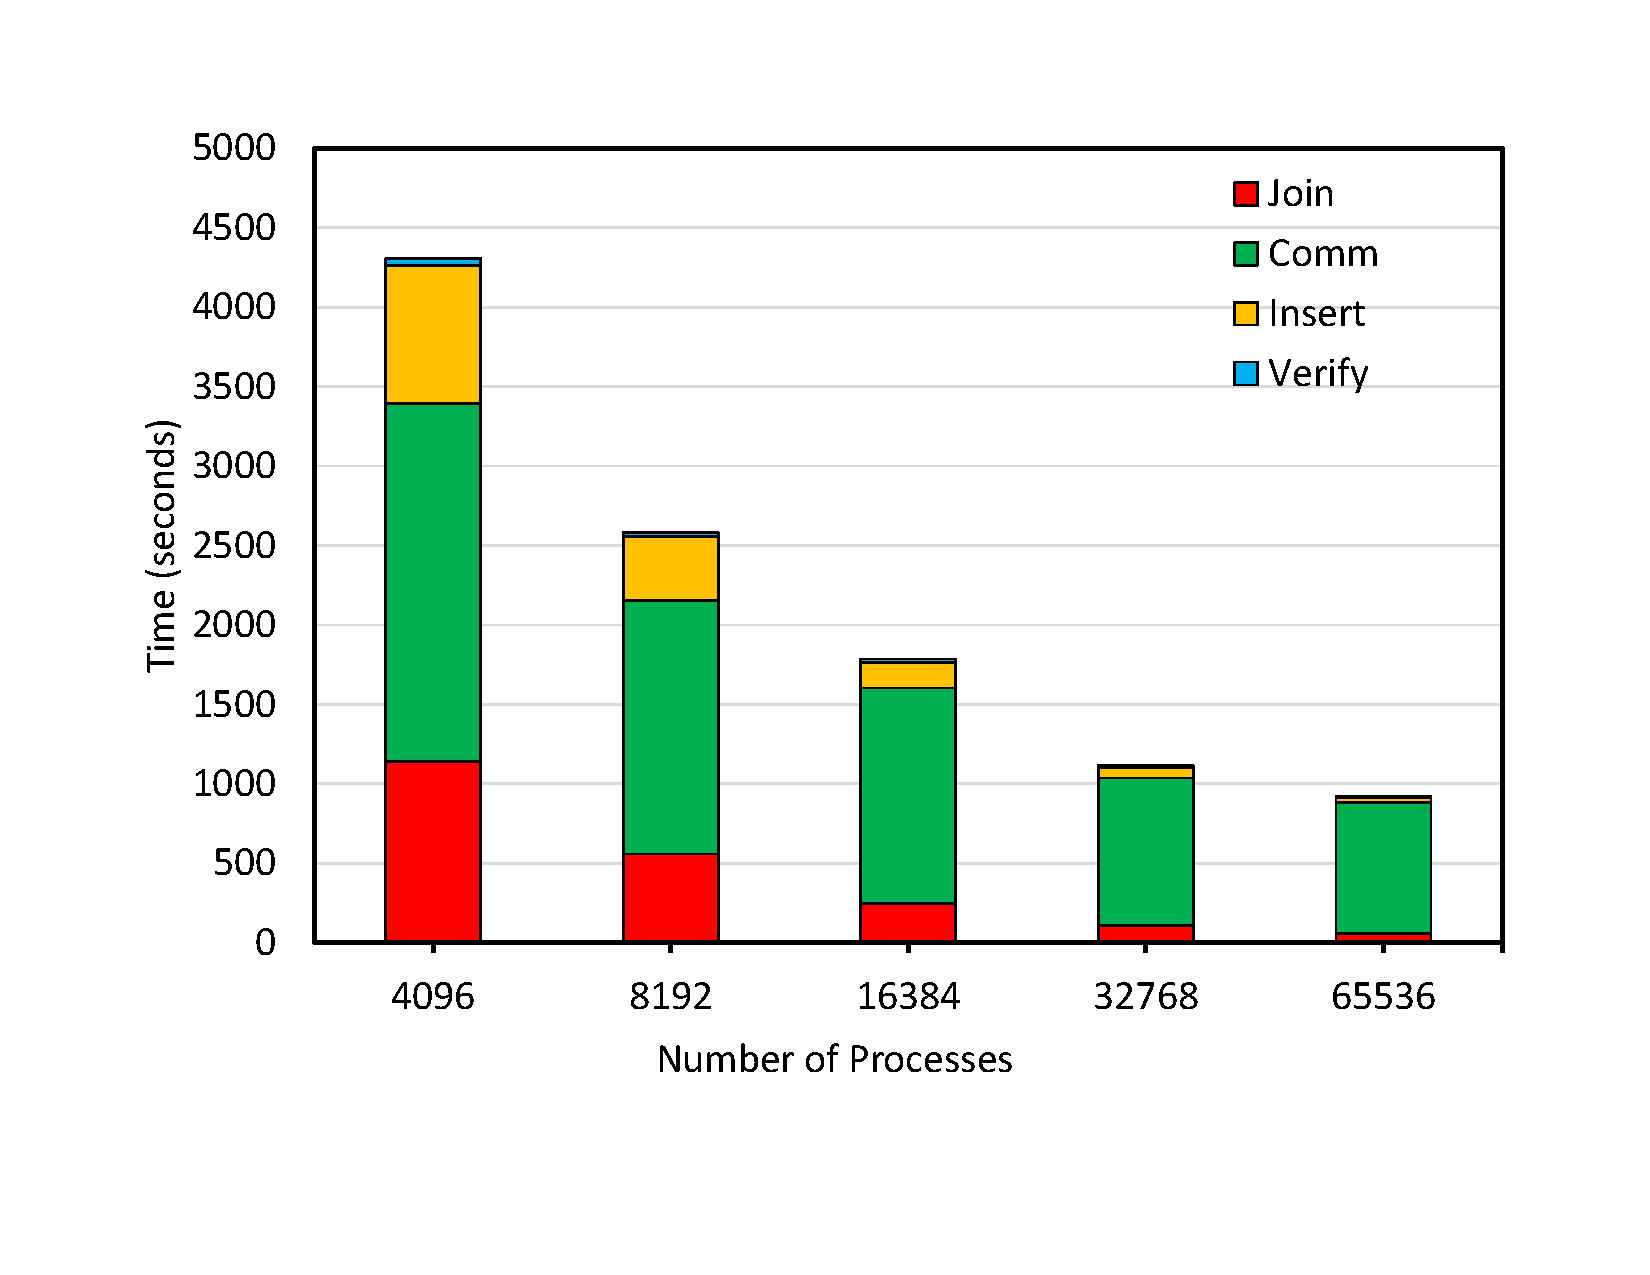
\includegraphics[width=.50\textwidth,  trim={0cm 0cm 0cm 0cm,
			clip}]{results/TC_260Billion_breakdown.pdf}}\hfill%
	\centering
	\caption{Transitive closure of a graph with X edges.}
	\label{fig:tc_large}
\end{figure*}